%\title{SWEETcam submission for IEEE Computer}

%%
%% Draft version 1.0
%%
%% Authors:
%% Kevin Abas
%% Caio Porto
%% Katia Obraczka 
%%

%% The template used was by Michael Shell
%% see http://www.michaelshell.org/
%% for current contact information.

%%*************************************************************************
%% Legal Notice:
%% This code is offered as-is without any warranty either expressed or
%% implied; without even the implied warranty of MERCHANTABILITY or
%% FITNESS FOR A PARTICULAR PURPOSE! 
%% User assumes all risk.
%% In no event shall IEEE or any contributor to this code be liable for
%% any damages or losses, including, but not limited to, incidental,
%% consequential, or any other damages, resulting from the use or misuse
%% of any information contained here.

%%*************************************************************************

\documentclass[journal,transmag]{IEEEtran}

% *** GRAPHICS RELATED PACKAGES ***
%
\usepackage{graphicx}
\ifCLASSINFOpdf

\else

\fi

% *** ALIGNMENT PACKAGES ***
%
\usepackage{array}

% *** PDF, URL AND HYPERLINK PACKAGES ***
%
\usepackage{url}
% url.sty was written by Donald Arseneau. It provides better support for
% handling and breaking URLs. url.sty is already installed on most LaTeX
% systems. The latest version and documentation can be obtained at:
% http://www.ctan.org/tex-archive/macros/latex/contrib/url/
% Basically, \url{my_url_here}.

% correct bad hyphenation here
\hyphenation{op-tical net-works semi-conduc-tor}

\begin{document}
%
% paper title
% can use linebreaks \\ within to get better formatting as desired
% Do not put math or special symbols in the title.
\title{Removing Physical Limits, \textsc{Secuirity cameras of the Future}}



% author names and affiliations
% transmag papers use the long conference author name format.

\author{\IEEEauthorblockN{Kevin Abas\IEEEauthorrefmark{1},
Caio Porto\IEEEauthorrefmark{2},
Katia Obraczka\IEEEauthorrefmark{1}}
\IEEEauthorblockA{\IEEEauthorrefmark{1}School of Engineering,
University of California Santa Cruz, CA 95064 USA}
\IEEEauthorblockA{\IEEEauthorrefmark{2}Escola Politecnica ´
Avenida Athos da Silveira Ramos ´
Rio de Janeiro, 21941-909, Brazil}
}

% for Transactions on Magnetics papers, we must declare the abstract and
% index terms PRIOR to the title within the \IEEEtitleabstractindextext
% IEEEtran command as these need to go into the title area created by
% \maketitle.
% As a general rule, do not put math, special symbols or citations
% in the abstract or keywords.
\IEEEtitleabstractindextext{%
\begin{abstract}
The abstract goes here.
\end{abstract}

% Note that keywords are not normally used for peerreview papers.
\begin{IEEEkeywords}
IEEEtran, journal, \LaTeX, magnetics, paper, template.
\end{IEEEkeywords}}



% make the title area
\maketitle

\IEEEdisplaynontitleabstractindextext

\IEEEpeerreviewmaketitle



\section{Introduction}
 
% Here we have the typical use of a "T" for an initial drop letter
% and "HIS" in caps to complete the first word.
\IEEEPARstart{T}{his} paper discusses ...

\subsection{Background, motivation} 
\-- Goals of the paper, What problems this papers solves \\

% needed in second column of first page if using \IEEEpubid
%\IEEEpubidadjcol

\subsubsection{Today's applications (summary)}
\-- Some things current Smart Camera networks assist with when it comes to 
surveillance and crime detection nodes. \\


\section{Requirements for today's wireless Smart Camera Networks}
\-- What are some more recent technologies being used and discovered by
researchers today. \\

\section{Wireless Smart Camera Networks Taxonomy}
\-- Purpose criteria for classification of wireless Smart camera networks \\ \\
\-- A comparison chart of different hardware components of their systems 
	being used\\ \\
\-- A comparison chart of software design features (computer vision, network
	topologies, bandwidth/energy saving techniques, etc. )\\ \\
\-- Explain each classification criterion, provide examples, etc.\\ \\

\section{Example Wireless Smart Camera Systems}
\-- Going into more detail of possibly one of the examples shown above in
	the taxonomy\\ \\
\--

\section{Our Project}

\subsection{Hardware}
 \-- Discuss breifly about the different components and why they were chosen \\

\subsubsection{WiFi 802.11n \\}
\subsubsection{MSP430 \\}

% needed in second column of first page if using \IEEEpubid
%\IEEEpubidadjcol

\subsection{Software}
\subsubsection{Image Processing}
\- Considering the constraints of the system in terms of price and hardware, it is used techniques of background subtraction to do the object detection. When started, the program keep taking pictures and process them using Mixture of Gaussian (MoG) method by Stauffer and Grimson. With the foreground in hands we find the contours and then a bounded box is applied following the contours' limit. To remove some noise and false detection a step is added to ignore objects of small size. The object classification is the most processor consumption  processes for most of the pedestrian detection systems, because it is used training techniques to classify the objects based on a previous stored database. In our case, to reduce the process we classify the objects by looking at their dimensions, they are classified as human if the height is two times bigger than the width we classify as a person. \\
\begin{figure}[h!]
\centering
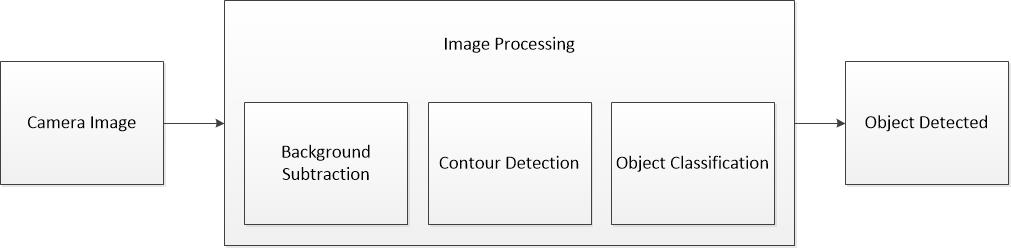
\includegraphics[scale=0.3]{imageprocessing}
\end{figure}	
\- This light system can generate some false alarms, but in association with the whole system, and its sensors, it can be improved for a better performance. There are other more robust object detection methods that could be used, but we would have a very low fps rate. \\
\- We developed using the Raspberry Pi camera module, which has already an API in C language and capable of capturing 1920x1080 resolution color images with 30 fps rate. For the image processing, we chose the Open Source Computer Vision Library (OpenCv). Our computer vision system is developed in C++ for better integration between the OpenCV and the API.\\

\subsection{Future Goals}

\section{Future Directions for Smart Wireless Camera Networks}
\-- Discuss research that has been proposed in the area and that is just begining to be implemented or hasn't yet at all.\\

\section{Conclusion}
\-- tie up paper

% use section* for acknowledgement
\section*{Acknowledgment}


\-- might not need this ...


% Can use something like this to put references on a page
% by themselves when using endfloat and the captionsoff option.
\ifCLASSOPTIONcaptionsoff
  \newpage
\fi

% references section

% can use a bibliography generated by BibTeX as a .bbl file
% BibTeX documentation can be easily obtained at:
% http://www.ctan.org/tex-archive/biblio/bibtex/contrib/doc/
% The IEEEtran BibTeX style support page is at:
% http://www.michaelshell.org/tex/ieeetran/bibtex/
%\bibliographystyle{IEEEtran}
% argument is your BibTeX string definitions and bibliography database(s)
%\bibliography{IEEEabrv,../bib/paper}
%
% <OR> manually copy in the resultant .bbl file
% set second argument of \begin to the number of references
% (used to reserve space for the reference number labels box)
\begin{thebibliography}{1}

\bibitem{IEEEhowto:kopka}
H.~Kopka and P.~W. Daly, \emph{A Guide to \LaTeX}, 3rd~ed.\hskip 1em plus
  0.5em minus 0.4em\relax Harlow, England: Addison-Wesley, 1999.

\end{thebibliography}


% if you will not have a photo at all:
\begin{IEEEbiographynophoto}{Kevin Abas}
Biography text here.
\end{IEEEbiographynophoto}

\begin{IEEEbiographynophoto}{Caio Porto}
Biography text here.
\end{IEEEbiographynophoto}

\end{document}





% *** MATH PACKAGES ***
%
%\usepackage[cmex10]{amsmath}
% A popular package from the American Mathematical Society that provides
% many useful and powerful commands for dealing with mathematics. If using
% it, be sure to load this package with the cmex10 option to ensure that
% only type 1 fonts will utilized at all point sizes. Without this option,
% it is possible that some math symbols, particularly those within
% footnotes, will be rendered in bitmap form which will result in a
% document that can not be IEEE Xplore compliant!
%
% Also, note that the amsmath package sets \interdisplaylinepenalty to 10000
% thus preventing page breaks from occurring within multiline equations. Use:
%\interdisplaylinepenalty=2500
% after loading amsmath to restore such page breaks as IEEEtran.cls normally
% does. amsmath.sty is already installed on most LaTeX systems. The latest
% version and documentation can be obtained at:
% http://www.ctan.org/tex-archive/macros/latex/required/amslatex/math/


% An example of a floating figure using the graphicx package.
% Note that \label must occur AFTER (or within) \caption.
% For figures, \caption should occur after the \includegraphics.
% Note that IEEEtran v1.7 and later has special internal code that
% is designed to preserve the operation of \label within \caption
% even when the captionsoff option is in effect. However, because
% of issues like this, it may be the safest practice to put all your
% \label just after \caption rather than within \caption{}.
%
% Reminder: the "draftcls" or "draftclsnofoot", not "draft", class
% option should be used if it is desired that the figures are to be
% displayed while in draft mode.
%
%\begin{figure}[!t]
%\centering
%\includegraphics[width=2.5in]{myfigure}
% where an .eps filename suffix will be assumed under latex, 
% and a .pdf suffix will be assumed for pdflatex; or what has been declared
% via \DeclareGraphicsExtensions.
%\caption{Simulation Results.}
%\label{fig_sim}
%\end{figure}

% Note that IEEE typically puts floats only at the top, even when this
% results in a large percentage of a column being occupied by floats.


% An example of a double column floating figure using two subfigures.
% (The subfig.sty package must be loaded for this to work.)
% The subfigure \label commands are set within each subfloat command,
% and the \label for the overall figure must come after \caption.
% \hfil is used as a separator to get equal spacing.
% Watch out that the combined width of all the subfigures on a 
% line do not exceed the text width or a line break will occur.
%
%\begin{figure*}[!t]
%\centering
%\subfloat[Case I]{\includegraphics[width=2.5in]{box}%
%\label{fig_first_case}}
%\hfil
%\subfloat[Case II]{\includegraphics[width=2.5in]{box}%
%\label{fig_second_case}}
%\caption{Simulation results.}
%\label{fig_sim}
%\end{figure*}
%
% Note that often IEEE papers with subfigures do not employ subfigure
% captions (using the optional argument to \subfloat[]), but instead will
% reference/describe all of them (a), (b), etc., within the main caption.


% An example of a floating table. Note that, for IEEE style tables, the 
% \caption command should come BEFORE the table. Table text will default to
% \footnotesize as IEEE normally uses this smaller font for tables.
% The \label must come after \caption as always.
%
%\begin{table}[!t]
%% increase table row spacing, adjust to taste
%\renewcommand{\arraystretch}{1.3}
% if using array.sty, it might be a good idea to tweak the value of
% \extrarowheight as needed to properly center the text within the cells
%\caption{An Example of a Table}
%\label{table_example}
%\centering
%% Some packages, such as MDW tools, offer better commands for making tables
%% than the plain LaTeX2e tabular which is used here.
%\begin{tabular}{|c||c|}
%\hline
%One & Two\\
%\hline
%Three & Four\\
%\hline
%\end{tabular}
%\end{table}


% Note that IEEE does not put floats in the very first column - or typically
% anywhere on the first page for that matter. Also, in-text middle ("here")
% positioning is not used. Most IEEE journals use top floats exclusively.
% Note that, LaTeX2e, unlike IEEE journals, places footnotes above bottom
% floats. This can be corrected via the \fnbelowfloat command of the
% stfloats package.






% if have a single appendix:
%\appendix[Proof of the Zonklar Equations]
% or
%\appendix  % for no appendix heading
% do not use \section anymore after \appendix, only \section*
% is possibly needed

% use appendices with more than one appendix
% then use \section to start each appendix
% you must declare a \section before using any
% \subsection or using \label (\appendices by itself
% starts a section numbered zero.)
%





% trigger a \newpage just before the given reference
% number - used to balance the columns on the last page
% adjust value as needed - may need to be readjusted if
% the document is modified later
%\IEEEtriggeratref{8}
% The "triggered" command can be changed if desired:
%\IEEEtriggercmd{\enlargethispage{-5in}}

